\chapter{A Physical Perspective on The Rescue of Mutant CFTR}
\label{chap:perspective}

\begin{chapquote}{Deborah Marcus ``Ouroboros'' \cite{marcus_ouroboros}}
and take the time to remember\\
the looping bend, surged\\
began as the walking end
\end{chapquote}

\section{Introduction}

The preceding chapters have fit into some broad themes. Chapters \ref{chap:introduction} and \ref{chap:methods} outlined a philosophy of biological physics. Meanwhile, chapters \ref{chap:cftr}-\ref{chap:opening} collected molecular details about the CFTR protein and its misfunction. This knowledge let us built up an understanding of the root cause of Cystic Fibrosis, and demonstrate that small molecule drugs can rescue diverse modes of CFTR misfunction. In this chapter we will tie these themes together. We will introduce a physical perspective on the rescue of mutant CFTR by potentiator drugs. However, a similar model could be built for corrector drugs, or even used to think about the modulation of any protein by small molecules.

We hope that this model will inform our current understanding of the action of CFTR modulators and also direct future efforts in treating the root cause of Cystic Fibrosis. The specific studies motivated by this model will be outlined in the next chapter.

In this chapter we will begin with a brief overview of our results so far, looking at the four CF-causing mutations we studied, which all responded to CFTR modulators even though they each had a unique molecular defect. We will then look at the molecular details of one of the best studied, and most common disease causing mutations, G551D.  
%, and where it fits in relation to the array of other disease causing mutations. 

We will show through simple unbiased MD that this mutation causes a disruption to the binding of ATP---resulting in a gating defect. As with previous chapters, this gating defect appears unique, sharing little in common with the other gating defects we analysed previously. This array of different disease phenotypes leads us to propose a physical model for the potentiating of mutant CFTR based on the underlying free energy landscape for the gating cycle. This model was formulated to explain the rescue of unique phenotypes by a common mechanism of action. 

At the end of this chapter we will demonstrate how to use our proposed model to theratype a rare mutation, Q1291H, from the molecular level. Our simulations suggest that Q1291H-CFTR exhibits a surprisingly similar mode of misfunction to the G551D defect, which responds to potentiators. Hence, it seems likely that the Q1291H mutation will also respond to these drugs. 

Despite this similar mode of pathogenesis patients carrying Q1291H-CFTR are excluded from receiving modulator therapy in all jurisdictions. Since Q1291H is such a rare mutation, its response to modulators has never been tested in model cell lines or in primary cell models. However, the \textit{in silico} analysis we present here would suggest that this mutation has a high likelihood to respond to modulators, demonstrating the power of a physical understanding of disease pathogenesis.

In the next chapter, we will use our proposed mechanistic model for the rescue of CFTR to suggest a direction for future studies into the molecular cause of CF. It is hoped that these future studies will collect the necessary quantitative information to fill in the missing information in our proposed model and assist in the development of a rational basis for the choice of CFTR modulators. 

%Our simulations of G551D and Q1291H appear to show a similar molecular phenotyope, even though they occur on different parts of the protein. Q1291H is an extremely rare mutation, it has not been clinicarlly characteriesd and is not approved for treatment with modulators. So, by studying a common mutation, G551D and comparing it to Q1291H we give an example of theratyping of CF mutations from the molecular level.


\section{Summary Of Rare Mutations Studied so Far}

	\begin{center}
	  \includegraphics[width=\textwidth]{figures/perspective/summary.pdf}
	\end{center}
\begingroup
\captionsetup{singlelinecheck = false, justification=raggedright}
\captionof {figure}[Summary of our Rare Mutation Studies] {\textbf{Summary of our Rare Mutation Studies}}{All of the mutations analysed in this thesis been largely unique. They occur on different domains of the CFTR protein and each cause misfunction through a unique set of molecular interactions. Nonetheless, all of these mutations responded, to some degree, to potentiator class modulators \cite{wong2022, wong2022a, kim2018, vanwilligen2019}. This situation demands that we tie together these results, to explain how different modes of pathogenesis can be treated by the same mechanism of action. } 
\label{summary_rare_mutations_MD}
\endgroup

In each of chapters \ref{chap:I37R}, \ref{chap:R352Q}, \ref{chap:S945L} and \ref{chap:opening}, we analysed a disease causing mutation in detail in order to understand \textit{how} it caused CFTR to misfunction. What these chapters have shown is a large diversity of molecular phenotypes. Each of these mutations appears to cause CFTR misfunction in a different way (Figure \ref{summary_rare_mutations_MD}). 

%In chapters \ref{chap:I37R}-\ref{chap:opening} we demonstrated that a diverse set of molecular defects respond to CFTR modulators. Each of these defects displayed a response to CFTR potentiators. This means that even though the molecular origin of pathogenesis was unique, each defect could be treated by a common mechanism of action. 

\begin{itemize}
	\item Chapter \ref{chap:I37R} studied the novel mutation I37R on the lasso motif. These results demonstrated that pathogenesis arises from interactions between the lasso motif and the R-domain. This caused a class III gating defect, which was responsive to both potentiators and some correctors \cite{wong2022}. 
	\item Chapter \ref{chap:R352Q} studied the R352Q mutation on TMD1, to show how a conductance class defect arose from the deletion of a positive charge in the inner vestibule of CFTR. This mutation was found to responded to potentiators \cite{wong2022a}.
\item Chapter \ref{chap:S945L} studied the S945L mutation on TMD2. Our simulations showed how a stable network of hydrogen bonds allows WT-CFTR to fold and gate correctly. When this set of hydrogen bonds was broken in S945L-CFTR, it led to class II and III folding and gating defects. This mutation was found to benefit from combination therapies, thus deriving some benefit from correctors as well as potentiators.  
\item Chapter \ref{chap:opening} studied the R334W mutation on TMD1. By using a dilated conformation of CFTR, we found that the deletion of a positive charge in the selectivity filter of CFTR lead to a class IV conductance defect. Previous studies in the literature demonstrated that this mutation also benefits from combination therapies, indicating that R334W-CFTR is amenable to modulation by both correctors and potentiators. 
\end{itemize}

Observe in the list above how each mutation causes misfunction in a different way. They occur in different parts of the CFTR protein and each had a different set molecular interactions which resulted in pathogenesis. What is thus remarkable is that the \textit{in vitro} evidence accompanying these computational studies all demonstrated that these mutations were responsive to the same modulators, albeit with differing efficacies. Each mutation we simulated responded to the mechanism of action of potentiators to some degree. These results, in combination with the knowledge that 174 other mutations have been shown to respond \textit{in vitro} to a combination therapy, lead us to expect that the majority of missense mutations will be amenable to treatment via CFTR modulators \cite{trikafta_FDA_info}. It is merely a problem of choosing the correct ones for each patient.

In order to help make these choices, here we will propose a rational basis for the action of potentiators. Hopefully, once developed further, this model can be used to conceptualise the mechanism of action for CFTR modulators and eventually, quantitatively predict whether a mutation will respond to a given modulator. In the next chapter we will outline the necessary steps for future studies to complete this model. 

In this chapter we will demonstrate the application of this rational basis. By briefly studying a common class III gating mutation, G551D, and how it fits into the overall classification of CF-causing mutations. We will then use our proposed model to compare the G551D mutation to a rarer mutation, Q1291H, which leads us to predict that they will both respond to the same modulators. 

\section{Simulating the Common G551D Gating Mutation}

	\begin{center}
		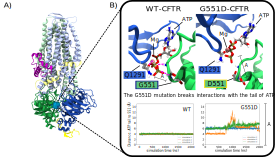
\includegraphics[width=\textwidth]{figures/perspective/G551D.pdf}
	\end{center}

\begingroup
\captionsetup{singlelinecheck = false, justification=raggedright}
\captionof {figure}[Pathogenesis in G551D-CFTR] {\textbf{Pathogenesis in G551D-CFTR}}{G551D-CFTR exhibits the prototypical gating phenotype \textit{in vitro} \cite{bompadre2007, wang2020}. A) The mutation is located on NBD1, in the vicinity of site 2, the hydrolytic ATP+Mg binding site. B) In WT-CFTR, the amide groups on the backbone of G550 and G551 stabilize the phosphate tail of the bound ATP molecule via hydrogen bonds. These links were found to be disrupted in simulations of G551D-CFTR. We propose that this means that G551D-CFTR has a lower binding affinity for ATP, giving rise to a gating defect.} 
\label{G551D_results}
\endgroup

Here, we will briefly continue the theme of previous chapters, with a simple MD study to understand pathogenesis in a common class III gating mutation, G551D \cite{li1996}. This will place the mutation in context with the rest of our work. This gating mutation occurs in NBD1, a domain we have not yet studied in the work of this thesis (Figure \ref{G551D_results}A). The G551D mutation holds historic importance in the study of CFTR, as it was the platform for the high-throughput screening which discovered potentiator class drugs \cite{vangoor2009}. This also means that G551D is a good candidate for comparison with other rare mutations if we wish to find other mutations which might also respond to potentiators.

Through MD simulations of WT-CFTR, it was found that G550 and G551 contributed critical hydrogen bonds when binding the phosphate tail of ATP in site 2. Upon mutation to G551D, this binding mode was disrupted, indicating the mutant will have lower binding affinity for binding ATP at this site (Figure \ref{G551D_results}B). Given the importance of ATP binding to the gating cycle of CFTR, these observations were a clear, rational basis for the confirmation of the G551D mutation as a class III gating defect \cite{bompadre2008}. Again, this molecular defect appears unique compared to those we have studied previously. None of the other mutations we have seen caused misfunction in this way. Nonetheless, the G551D mutation \textit{also} responds to CFTR potentiators \cite{vangoor2009,wong2022a,kalydeco_FDA_approval}. 

The number and diversity of gating defects we have characterised raises some issues. Clearly, several types of misfunction may be classified as gating defects, many of which respond to potentiators. The complexity of this situation suggests that the class III category of defects is actually made up of several sub classes. In the next section, we will take a broader view. We will use the physical understanding of CFTR which we have built up in the preceeding chapters in order to survey the literature to build more meaningful classes of CFTR misfunction.

\section{The Many Molecular Modes of Misfunction in CFTR}

Throughout the literature and this thesis, we have seen many different many modes of misfunction in CFTR and each one we studied seems distinct. Hence, it is unlikely that the classification of mutations into six broad classes can be used to theratype patients with precision \cite{veit2016}. A molecular understanding of CFTR misfunction is needed to choose modulators which will optimally rescue each mutation.

In Figure \ref{granular_classification} we have surveyed the available literature to sketch out a more complete, more granular classification of different mutations. Observe in this figure how we have identified 16 different structural and functional modes of CFTR misfunction. These classes themselves are quite broad. For example the category ``NBD folding" contains dozens of mutations not listed---F575Y, S492F, R560S, R1066C and S1128F to name a few \cite{awatade2019, lopes-pacheco2016, casals1997, cotten1996, penmatsa2009}. As before, each of these mutations likely have their own characteristic molecular fingerprints which result in pathogenesis. It will take some work to split up this category further, to make it more meaningful when choosing modulators targeting specific mutations.

The complexity in Figure \ref{granular_classification} shows some of the nuance within CF pathogenesis. In order to make this summary more manageable and more meaningful, in the next section we will propose a physical model with which to understand the modulation of gating class CFTR mutants. Using this model we will then show how it may be used to suggest modulators to treat a rare mutation.

\begin{landscape}
\begin{figure}
	\begin{center}
	%\includegraphics[angle=270,origin=c,width=0.38\textwidth]{figures/classes_mutations.pdf}\\
	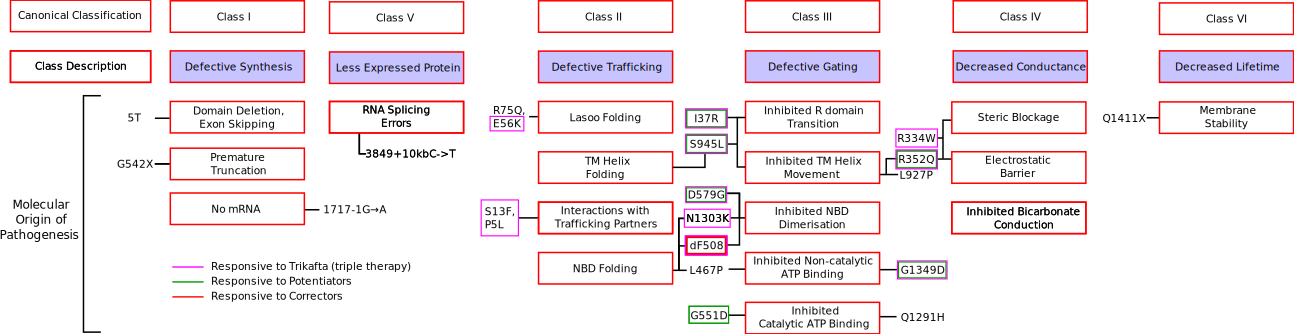
\includegraphics[width=1.5\textwidth]{figures/perspective/classes_mutations.pdf}\\
	\end{center}
	\captionsetup{singlelinecheck = false, justification=raggedright}
	\caption[Granular grouping of CF pathogenesis]{\textbf{Granular Grouping of Cystic Fibrosis Causing Mutations}{ Conventionally, molecular CF phenotypes are grouped into 6 classes. These classes, while useful in a clinic, are quite broad. They struggle to reflect that molecular misfunction can arise from many different interactions within CFTR. By realising that classification into a given class can be due to different factors, we can gain a more complete picture of the molecular cause of CF. The links drawn in this figure were inferred from a combination of sources in the literature, our own findings and from a mutation's location in the CFTR protein \cite{bompadre2007, yeh2019a, gong2004, wong2022, vangoor2009, vangoor2014, hoffmann2018, thelin2007, gene2008, trikafta_website, phuan2018, ensinck2022}. The inhibited bicarbonate conductance class was included to highlight that there are few molecular studies which have sought to understand the molecular effects of different mutations on the conduction of bicarbonate, despite its important role in disease pathogenesis. }
	}

	\label{granular_classification}
\end{figure}
\end{landscape}

\section{A Physics Motivated Approach to Personalised Medicine in Cystic Fibrosis}
Observe in Figure \ref{granular_classification} how mutations which cause misfunction in different ways may respond to the same modulators. 

For example, as we have shown in detail I37R and G551D occur on different domains of CFTR, resulting in different kinds of pathogenesis. Despite this, they can both be rescued by the potentiator class drug ivacaftor (VX770) \cite{vangoor2014,wong2022}. In order to explain these results, and the observation that even WT-CFTR is modulated by potentiators \cite{csanady2019}, in this chapter we will propose a conceptual framework which explains how these drugs are able to treat such diverse molecular phenotypes. This model would appear to suggest that patients with rare missense mutations are likely respond to the right choice of CFTR modulators. This model may also inform the design of future CFTR modulators and this will be discussed in the next chapter. 

\begin{figure}
	\begin{center}
		\begingroup
	
\includegraphics[width=0.6\textwidth]{figures/perspective/drug_landscape_1.pdf}\\
	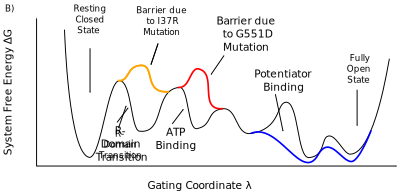
\includegraphics[width=0.6\textwidth]{figures/perspective/drug_landscape_3.pdf}\\
		\endgroup
	\end{center}
	\begingroup
	\captionsetup{singlelinecheck = false, justification=raggedright}
	\captionof{figure}[Conceptual Framework for the Pathogenesis of Mutations and The Action of Potentiators]{\textbf{Conceptual Framework for the Pathogenesis of Mutations and The Action of Potentiators}{ A) The transition between the resting closed state and fully open state of CFTR can be visualised as a movement through an energy landscape. During this transition various events must occur, such as the movement of the R-domain, ATP-binding and the movement of the TMDs to form a pore. Each of these events will have an energetic cost and payoff, giving rise to peaks and troughs in the energy landscape of the transition. The relative heights of peaks and troughs here are for illustrative purposes only, but quantitative techniques to calculate them will have important implications for the treatment of CF and drug discovery. B) Gating class CF-causing mutations give rise to pathogenic barriers in this energy landscape which prevent the transition to an open state. They may arise in different parts of the energy landscape. For example, we have shown that G551D causes a disruption to the binding of ATP, while in chapter \ref{chap:I37R}, we saw a gating defect arise in I37R-CFTR from the misregulation of the position of the R-domain. This demonstrates how pathogenesis can arise in many different ways in CFTR. Furthermore, accompanying \textit{in vitro} studies of these mutations demonstrated that these unique mutations each respond to potentiator class modulators. This indicates that CFTR potentiators are bringing down \textit{other} barriers in this energy landscape in order to compensate for these mutations. By understanding \textit{where} mutations are causing gating inhibition and \textit{how} drugs are accounting for the deleterious energetics, we can begin to build a molecular basis for the choice of modulators, tailored to each mutation.}}
	\label{drug_action_model}

	\endgroup
\end{figure}

The model in Figure \ref {drug_action_model} has been proposed to explain the action of potentiators in the treatment of gating defects. It was formulated with this focus because the gating transition of CFTR is well understood. There are many well studied events which we can visualise in our model energy landscape--like ATP binding and pore formation by the TMDs. Hence, we have built our model with a focus on this aspect of protein function. Nonetheless, the conceptual basis of this model is transferable to CFTR folding and the action of correctors as well, once we elucidate more of the folding pathway \cite{krainer2018, kleizen2021, kleizen2020, padanyi2022, fiedorczuk2022}. 

Currently, a range of missense mutations are recommended for treatment by various modulator therapies, but many more are excluded from receiving these treatments due to a lack of testing \cite{trikafta_FDA_info, kalydeco_FDA_approval, vangoor2014}. With an understanding of the root cause of disease in these missense mutations, their exclusion from receiving modulator therapy seems strange.

From the perspective of protein physics, the more common and well studied $\Delta$F508 mutation causes a much greater defect to CFTR than the majority missense mutations \cite{bahia2021}. Hence, we would expect almost every missense mutation would respond to modulator therapy. In this way it makes little sense not to screen patients carrying missense mutations for a response to modulators. 

From our simulation results and the model in Figure \ref{drug_action_model}, we propose that when a given patient does not respond to modulators, it is likely due to the underlying cellular factors which gives rise to the heterogeneous response to modulators found across all CF patients \cite{boyle2014, donaldson2018, keating2018, matthes2018}. There is little reason to suspect that the drugs are failing to act on the mutation at the molecular level. Hence, the pre-clinical, patient specific approach like the one employed by the collaborators of this thesis is most appropriate for the treatment of CF. 

%It is still likely that many of these patients may not respond to modulators. However, from our simulation results and the model in Figure \ref{drug_action_model}, it seems likely that that the lack of a response in a given patient is due to the broader heterogeneous response to modulators found in many CF patients \cite{boyle2014, donaldson2018, keating2018, matthes2018}---as opposed to the failure of modulators to act on a given mutation. Hence, the pre-clinical, patient specific approach like the one employed by the collaborators of this thesis is most appropriate for the treatment of CF. 

Our simulations have aided this personalised effort, by demonstrating that a wide range of defects are amenable to pharmacological rescue. We will now go one step further, by showing how an atomistic understanding of CFTR can be used to theratype a rare mutation. We have specifically chosen a poorly studied mutation from our dataset, to demonstrate the capability of the model we now have in hand. 

\section{Theratyping Q1291H-CFTR With Atomic Precision}

Through our MD simulations, we noticed another mutation, Q1291H, appears to produce a similar molecular defect to G551D-CFTR. This was a little bit surprising, as the Q1291H mutation is located on a different domain of CFTR to G551D (NBD2 as opposed to NBD1). G551D is much more common than Q1291H, and so patients carrying the former may access potentiators. However, Q1291H is extremely rare only---30 alleles with this mutation have been recorded in the CFTR2 database. This mutation is also poorly understood clinically, as it can result in a variety of outcomes for the patient \cite{cftr2}. Our study of this mutation was also motivated by the fact that samples with this mutation are in the biobank of Sydney Children's hospital, taken from a CF afflicted patient. 

Because of their heterozygous alleles and the rarity of the Q1291H mutation, this patient is currently excluded from receiving modulator therapy. As with our previous studies, we propose that computational results can compliment, and in this case, predict the results of patient specific \textit{in vitro} assays. 

The Q1291H mutation is located on NBD2 (Figure \ref{Q1291H_results}A). In WT-CFTR simulations, we noticed that the oxygen atom in the  Q1291 sidechain made a stable contact with the magnesium cofactor of ATP in site 2. This interaction will contribute to the high binding affinity of site 2 for its ATP and magnesium. 

Hence, it was not surprising to see this interaction broken upon mutation. During mutations to both histidine and phenylalanine, we noticed that both the G550 and G551 interactions were broken, as in the G551D-CFTR simulations, and the amino acid at position 1291 moved away from magnesium (Figure \ref{Q1291H_results}B). This indicated a disruption to the binding of ATP at site 2. 

In the case of Q1291H-CFTR the breaking of this interaction was unreliable due to the polar histidine side chain. However, comparison another mutation, Q1291F, which does not poses a polar side chain confirmed the presence of this defect. This logic is also supported by \textit{in vitro} experiments, where the Q1291F mutation exhibits a very similar gating phenotype to Q1291H \cite{dong2015}. 

These results show that both G551D and Q1291H disrupt ATP binding at site 2. Further, since we know that this kind of dysfunction is amenable to rescue by CFTR modulators in the case of G551D, we would expect that Q1291H-CFTR would also respond to potentiators or combination therapy. This is shown in Figure \ref{Q1291H_results}C, where the deleterious barriers from G551D and Q1291H are drawn at similar positions in the energy landscape. Should these mutations produce similar defects they should \textit{also} respond to similar modulators.

Our recommendations for the Q1291H mutation are further strengthened by the fact that another mutation at the 1291 position, Q1291R, has been tested in \textit{in vitro} assays and is now recommended, by the US Food and Drug Administration, for treatment by both potentiators and combination therapies \cite{trikafta_website, trikafta_FDA_info, kalydeco_FDA_approval}. Given that the Q1291R mutation introduces a charge into the protein, it is likely to be more deleterious than Q1291H---note that the latter mutation is charge neutral. In the next iteration of the above study, we will also add Q1291R to our dataset. 

Although computational modelling is not sufficiently advanced to make a recommendation for any patient without \textit{in vitro} studies, the situation of the patient carrying the Q1291H mutation is common for those with rare forms of CF. So, we recommend that this mutation be tested in patient specific assays, as the results have a high likelihood to translate to clinical practice. This would prove the utility of the mechanistic understanding we are attempting to deliver---to compliment existing patient specific platforms.


%There is no reason to beleive that even in patients who do not show benefit from modulator therapy that the drugs are for some reason not reaching the CFTR protein. In fact, they seem to metabolise the drugs at teh same rate as patients who do. The success of preclinical models indicates that the problem is the cellular level and not at the level of organs or tissues. There is probably some genetic or cellular component that has not yet been identified which, once addressed, could bring the benefits of modulators to these patients.

\begin{figure}
	\begin{center}
		\includegraphics[width=\textwidth]{figures/perspective/Q1291.pdf}
	\end{center}
	\captionsetup{singlelinecheck = false, justification=raggedright}
	\caption[Pathogenesis in Q1291H-CFTR]{\textbf{Pathogenesis in Q1291H-CFTR}{A) The Q1291H mutation occurs on NBD2, in the vicinity the catalytic ATP binding site, site 2. B) It appears as though this mutation also causes disruption to the binding of this ATP molecule, much like G551D. Data from simulations Q1291F is also included, as it more reliably produces the molecular perturbation which we expect is characteristic of the Q1291H mutation. \textit{In vitro}, the two mutations produce similar behaviour, and this is confirmed in our simulations \cite{dong2015}. }}

	\label{Q1291H_results}

\end{figure}


%These drugs are clinically efficacious \cite{vangoor2014} on several mutants with some curious exceptions like N1303K. I suggest the following mechanism for their action. I suspect a similar analogy exists for the action of the correctors. WT-CFTR exhibits a natural landscape with kinetic barriers in the transition between the closed and open states. A gating class mutation to CFTR will introduce a kinetic barrier in the pathway of this conformational transition. What these drugs do is reduce a barrier in the existing conformational landscape of CFTR. This compensates for the barriers introduced by the mutation. j


\section{Summary}
The preceding chapters have given technical and molecular details regarding the cause of Cystic Fibrosis due to rare genetic mutations. Further, by collaborating closely with cell biologists and clinicians, we have demonstrated that many molecular defects caused by mutations can be treated by existing small molecule drugs. The unique molecular fingerprint of each mutation we have studied is an indication that the best outcomes can be delivered to patients with a personalised approach to the choice of medication. 

In each of the four preceding chapters, we performed extensive MD simulations and free energy calculations in order to discover four very diverse modes of CFTR pathogenesis. In this chapter, in combination with the available literature and the presented study of G551D, we have proposed a model for the rescue of gating class mutations by potentiators. This model sought to account for the fact that we have seen many unique defects all responding to potentiator drugs. We also expect that a similar model could be formulated for folding defects and the action of correctors, once further studies of CFTR are completed. 

Our simulations results suggest that the majority of rare missense mutations will respond to modulator therapy---even though they are currently excluded from these treatments due to a lack of clinical data or well accepted pre-clinical model. We presented a short study of Q1291H-CFTR in to demonstrate an example of this problem. 

The findings of this thesis have demonstrated that the patient specific approach employed by our collaborators are effective tools to measure the outcomes in the treatment of modulators for several different CFTR phenotypes. Patients should thus be systematically theratyped with this approach, such that they can be screened for a response to an array of modulators. To further compliment these theratyping efforts, we will give some recommendations for a set of \textit{in silico} studies in the next chapter. The intention with these studies is that they perform the necessary work to complete our proposed model for the action CFTR modulators and  increase its predictive power.

%Since the identification of CFTR as the gene which causes disease, several disease causing mutations have been discovered in discovered in populations with low rates of Cystic Fibrosis. The genotypes in these populations is more likely to be rare, highlighting the need for a more personalised approach for these populations \cite{singh2015, zietkiewicz2014}.


\section{Method Details}
The simulation methodologies employed in this chapter were identical to those employed in chapter \ref{chap:S945L}. All MD simulations in this chapter were carried out at a physiological temperature of 310K (37$^o$C).
